% Options for packages loaded elsewhere
\PassOptionsToPackage{unicode}{hyperref}
\PassOptionsToPackage{hyphens}{url}
%
\documentclass[
]{article}
\usepackage{amsmath,amssymb}
\usepackage{lmodern}
\usepackage{ifxetex,ifluatex}
\ifnum 0\ifxetex 1\fi\ifluatex 1\fi=0 % if pdftex
  \usepackage[T1]{fontenc}
  \usepackage[utf8]{inputenc}
  \usepackage{textcomp} % provide euro and other symbols
\else % if luatex or xetex
  \usepackage{unicode-math}
  \defaultfontfeatures{Scale=MatchLowercase}
  \defaultfontfeatures[\rmfamily]{Ligatures=TeX,Scale=1}
\fi
% Use upquote if available, for straight quotes in verbatim environments
\IfFileExists{upquote.sty}{\usepackage{upquote}}{}
\IfFileExists{microtype.sty}{% use microtype if available
  \usepackage[]{microtype}
  \UseMicrotypeSet[protrusion]{basicmath} % disable protrusion for tt fonts
}{}
\makeatletter
\@ifundefined{KOMAClassName}{% if non-KOMA class
  \IfFileExists{parskip.sty}{%
    \usepackage{parskip}
  }{% else
    \setlength{\parindent}{0pt}
    \setlength{\parskip}{6pt plus 2pt minus 1pt}}
}{% if KOMA class
  \KOMAoptions{parskip=half}}
\makeatother
\usepackage{xcolor}
\IfFileExists{xurl.sty}{\usepackage{xurl}}{} % add URL line breaks if available
\IfFileExists{bookmark.sty}{\usepackage{bookmark}}{\usepackage{hyperref}}
\hypersetup{
  pdftitle={Class 10},
  pdfauthor={Claire Chapman},
  hidelinks,
  pdfcreator={LaTeX via pandoc}}
\urlstyle{same} % disable monospaced font for URLs
\usepackage[margin=1in]{geometry}
\usepackage{color}
\usepackage{fancyvrb}
\newcommand{\VerbBar}{|}
\newcommand{\VERB}{\Verb[commandchars=\\\{\}]}
\DefineVerbatimEnvironment{Highlighting}{Verbatim}{commandchars=\\\{\}}
% Add ',fontsize=\small' for more characters per line
\usepackage{framed}
\definecolor{shadecolor}{RGB}{248,248,248}
\newenvironment{Shaded}{\begin{snugshade}}{\end{snugshade}}
\newcommand{\AlertTok}[1]{\textcolor[rgb]{0.94,0.16,0.16}{#1}}
\newcommand{\AnnotationTok}[1]{\textcolor[rgb]{0.56,0.35,0.01}{\textbf{\textit{#1}}}}
\newcommand{\AttributeTok}[1]{\textcolor[rgb]{0.77,0.63,0.00}{#1}}
\newcommand{\BaseNTok}[1]{\textcolor[rgb]{0.00,0.00,0.81}{#1}}
\newcommand{\BuiltInTok}[1]{#1}
\newcommand{\CharTok}[1]{\textcolor[rgb]{0.31,0.60,0.02}{#1}}
\newcommand{\CommentTok}[1]{\textcolor[rgb]{0.56,0.35,0.01}{\textit{#1}}}
\newcommand{\CommentVarTok}[1]{\textcolor[rgb]{0.56,0.35,0.01}{\textbf{\textit{#1}}}}
\newcommand{\ConstantTok}[1]{\textcolor[rgb]{0.00,0.00,0.00}{#1}}
\newcommand{\ControlFlowTok}[1]{\textcolor[rgb]{0.13,0.29,0.53}{\textbf{#1}}}
\newcommand{\DataTypeTok}[1]{\textcolor[rgb]{0.13,0.29,0.53}{#1}}
\newcommand{\DecValTok}[1]{\textcolor[rgb]{0.00,0.00,0.81}{#1}}
\newcommand{\DocumentationTok}[1]{\textcolor[rgb]{0.56,0.35,0.01}{\textbf{\textit{#1}}}}
\newcommand{\ErrorTok}[1]{\textcolor[rgb]{0.64,0.00,0.00}{\textbf{#1}}}
\newcommand{\ExtensionTok}[1]{#1}
\newcommand{\FloatTok}[1]{\textcolor[rgb]{0.00,0.00,0.81}{#1}}
\newcommand{\FunctionTok}[1]{\textcolor[rgb]{0.00,0.00,0.00}{#1}}
\newcommand{\ImportTok}[1]{#1}
\newcommand{\InformationTok}[1]{\textcolor[rgb]{0.56,0.35,0.01}{\textbf{\textit{#1}}}}
\newcommand{\KeywordTok}[1]{\textcolor[rgb]{0.13,0.29,0.53}{\textbf{#1}}}
\newcommand{\NormalTok}[1]{#1}
\newcommand{\OperatorTok}[1]{\textcolor[rgb]{0.81,0.36,0.00}{\textbf{#1}}}
\newcommand{\OtherTok}[1]{\textcolor[rgb]{0.56,0.35,0.01}{#1}}
\newcommand{\PreprocessorTok}[1]{\textcolor[rgb]{0.56,0.35,0.01}{\textit{#1}}}
\newcommand{\RegionMarkerTok}[1]{#1}
\newcommand{\SpecialCharTok}[1]{\textcolor[rgb]{0.00,0.00,0.00}{#1}}
\newcommand{\SpecialStringTok}[1]{\textcolor[rgb]{0.31,0.60,0.02}{#1}}
\newcommand{\StringTok}[1]{\textcolor[rgb]{0.31,0.60,0.02}{#1}}
\newcommand{\VariableTok}[1]{\textcolor[rgb]{0.00,0.00,0.00}{#1}}
\newcommand{\VerbatimStringTok}[1]{\textcolor[rgb]{0.31,0.60,0.02}{#1}}
\newcommand{\WarningTok}[1]{\textcolor[rgb]{0.56,0.35,0.01}{\textbf{\textit{#1}}}}
\usepackage{longtable,booktabs,array}
\usepackage{calc} % for calculating minipage widths
% Correct order of tables after \paragraph or \subparagraph
\usepackage{etoolbox}
\makeatletter
\patchcmd\longtable{\par}{\if@noskipsec\mbox{}\fi\par}{}{}
\makeatother
% Allow footnotes in longtable head/foot
\IfFileExists{footnotehyper.sty}{\usepackage{footnotehyper}}{\usepackage{footnote}}
\makesavenoteenv{longtable}
\usepackage{graphicx}
\makeatletter
\def\maxwidth{\ifdim\Gin@nat@width>\linewidth\linewidth\else\Gin@nat@width\fi}
\def\maxheight{\ifdim\Gin@nat@height>\textheight\textheight\else\Gin@nat@height\fi}
\makeatother
% Scale images if necessary, so that they will not overflow the page
% margins by default, and it is still possible to overwrite the defaults
% using explicit options in \includegraphics[width, height, ...]{}
\setkeys{Gin}{width=\maxwidth,height=\maxheight,keepaspectratio}
% Set default figure placement to htbp
\makeatletter
\def\fps@figure{htbp}
\makeatother
\setlength{\emergencystretch}{3em} % prevent overfull lines
\providecommand{\tightlist}{%
  \setlength{\itemsep}{0pt}\setlength{\parskip}{0pt}}
\setcounter{secnumdepth}{-\maxdimen} % remove section numbering
\ifluatex
  \usepackage{selnolig}  % disable illegal ligatures
\fi

\title{Class 10}
\author{Claire Chapman}
\date{10/29/2021}

\begin{document}
\maketitle

\begin{Shaded}
\begin{Highlighting}[]
\NormalTok{url }\OtherTok{\textless{}{-}} \StringTok{"https://raw.githubusercontent.com/fivethirtyeight/data/master/candy{-}power{-}ranking/candy{-}data.csv"}
\NormalTok{candy\_file }\OtherTok{\textless{}{-}} \FunctionTok{read.csv}\NormalTok{(url)}
\NormalTok{candy }\OtherTok{=} \FunctionTok{data.frame}\NormalTok{(candy\_file, }\AttributeTok{row.names =} \DecValTok{1}\NormalTok{)}
\FunctionTok{head}\NormalTok{(candy)}
\end{Highlighting}
\end{Shaded}

\begin{verbatim}
##              chocolate fruity caramel peanutyalmondy nougat crispedricewafer
## 100 Grand            1      0       1              0      0                1
## 3 Musketeers         1      0       0              0      1                0
## One dime             0      0       0              0      0                0
## One quarter          0      0       0              0      0                0
## Air Heads            0      1       0              0      0                0
## Almond Joy           1      0       0              1      0                0
##              hard bar pluribus sugarpercent pricepercent winpercent
## 100 Grand       0   1        0        0.732        0.860   66.97173
## 3 Musketeers    0   1        0        0.604        0.511   67.60294
## One dime        0   0        0        0.011        0.116   32.26109
## One quarter     0   0        0        0.011        0.511   46.11650
## Air Heads       0   0        0        0.906        0.511   52.34146
## Almond Joy      0   1        0        0.465        0.767   50.34755
\end{verbatim}

\hypertarget{exploring-the-dataset}{%
\subsection{Exploring the dataset}\label{exploring-the-dataset}}

\begin{quote}
Q1. How many different candy types are in this dataset?
\end{quote}

\begin{Shaded}
\begin{Highlighting}[]
\FunctionTok{nrow}\NormalTok{(candy)}
\end{Highlighting}
\end{Shaded}

\begin{verbatim}
## [1] 85
\end{verbatim}

There are 85 types of candy in this dataset

\begin{quote}
Q2. How many fruity candy types are in the dataset?
\end{quote}

\begin{Shaded}
\begin{Highlighting}[]
\FunctionTok{sum}\NormalTok{(candy}\SpecialCharTok{$}\NormalTok{fruity)}
\end{Highlighting}
\end{Shaded}

\begin{verbatim}
## [1] 38
\end{verbatim}

38 fruity candy types

\hypertarget{what-is-your-favorite-candy}{%
\subsection{What is your favorite
candy?}\label{what-is-your-favorite-candy}}

winpercent is a value that tells, for a given candy, the percentage of
people that preferred that candy over another randomly chosen candy.
Extract winpercent of twix

\begin{Shaded}
\begin{Highlighting}[]
\NormalTok{candy[}\StringTok{"Twix"}\NormalTok{, ]}\SpecialCharTok{$}\NormalTok{winpercent}
\end{Highlighting}
\end{Shaded}

\begin{verbatim}
## [1] 81.64291
\end{verbatim}

\begin{quote}
Q3. What is your favorite candy in the dataset and what is it's
winpercent value?
\end{quote}

\begin{Shaded}
\begin{Highlighting}[]
\NormalTok{candy[}\StringTok{"Haribo Gold Bears"}\NormalTok{,]}\SpecialCharTok{$}\NormalTok{winpercent}
\end{Highlighting}
\end{Shaded}

\begin{verbatim}
## [1] 57.11974
\end{verbatim}

\begin{quote}
Q4. What is the winpercent value for ``Kit Kat''?
\end{quote}

\begin{Shaded}
\begin{Highlighting}[]
\NormalTok{candy[}\StringTok{"Kit Kat"}\NormalTok{,]}\SpecialCharTok{$}\NormalTok{winpercent}
\end{Highlighting}
\end{Shaded}

\begin{verbatim}
## [1] 76.7686
\end{verbatim}

\begin{quote}
Q5. What is the winpercent value for ``Tootsie Roll Snack Bars''?
\end{quote}

\begin{Shaded}
\begin{Highlighting}[]
\NormalTok{candy[}\StringTok{"Tootsie Roll Snack Bars"}\NormalTok{,]}\SpecialCharTok{$}\NormalTok{winpercent}
\end{Highlighting}
\end{Shaded}

\begin{verbatim}
## [1] 49.6535
\end{verbatim}

\textbf{skim()} function can help give a quick overview of a dataset

\begin{Shaded}
\begin{Highlighting}[]
\CommentTok{\#install.packages("skimr")}
\FunctionTok{library}\NormalTok{(}\StringTok{"skimr"}\NormalTok{)}
\FunctionTok{skim}\NormalTok{(candy)}
\end{Highlighting}
\end{Shaded}

\begin{longtable}[]{@{}ll@{}}
\caption{Data summary}\tabularnewline
\toprule
& \\
\midrule
\endfirsthead
\toprule
& \\
\midrule
\endhead
Name & candy \\
Number of rows & 85 \\
Number of columns & 12 \\
\_\_\_\_\_\_\_\_\_\_\_\_\_\_\_\_\_\_\_\_\_\_\_ & \\
Column type frequency: & \\
numeric & 12 \\
\_\_\_\_\_\_\_\_\_\_\_\_\_\_\_\_\_\_\_\_\_\_\_\_ & \\
Group variables & None \\
\bottomrule
\end{longtable}

\textbf{Variable type: numeric}

\begin{longtable}[]{@{}lrrrrrrrrrl@{}}
\toprule
skim\_variable & n\_missing & complete\_rate & mean & sd & p0 & p25 &
p50 & p75 & p100 & hist \\
\midrule
\endhead
chocolate & 0 & 1 & 0.44 & 0.50 & 0.00 & 0.00 & 0.00 & 1.00 & 1.00 &
▇▁▁▁▆ \\
fruity & 0 & 1 & 0.45 & 0.50 & 0.00 & 0.00 & 0.00 & 1.00 & 1.00 &
▇▁▁▁▆ \\
caramel & 0 & 1 & 0.16 & 0.37 & 0.00 & 0.00 & 0.00 & 0.00 & 1.00 &
▇▁▁▁▂ \\
peanutyalmondy & 0 & 1 & 0.16 & 0.37 & 0.00 & 0.00 & 0.00 & 0.00 & 1.00
& ▇▁▁▁▂ \\
nougat & 0 & 1 & 0.08 & 0.28 & 0.00 & 0.00 & 0.00 & 0.00 & 1.00 &
▇▁▁▁▁ \\
crispedricewafer & 0 & 1 & 0.08 & 0.28 & 0.00 & 0.00 & 0.00 & 0.00 &
1.00 & ▇▁▁▁▁ \\
hard & 0 & 1 & 0.18 & 0.38 & 0.00 & 0.00 & 0.00 & 0.00 & 1.00 & ▇▁▁▁▂ \\
bar & 0 & 1 & 0.25 & 0.43 & 0.00 & 0.00 & 0.00 & 0.00 & 1.00 & ▇▁▁▁▂ \\
pluribus & 0 & 1 & 0.52 & 0.50 & 0.00 & 0.00 & 1.00 & 1.00 & 1.00 &
▇▁▁▁▇ \\
sugarpercent & 0 & 1 & 0.48 & 0.28 & 0.01 & 0.22 & 0.47 & 0.73 & 0.99 &
▇▇▇▇▆ \\
pricepercent & 0 & 1 & 0.47 & 0.29 & 0.01 & 0.26 & 0.47 & 0.65 & 0.98 &
▇▇▇▇▆ \\
winpercent & 0 & 1 & 50.32 & 14.71 & 22.45 & 39.14 & 47.83 & 59.86 &
84.18 & ▃▇▆▅▂ \\
\bottomrule
\end{longtable}

\begin{quote}
Q6. Is there any variable/column that looks to be on a different scale
to the majority of the other columns in the dataset?
\end{quote}

The winpercent column looks to be on a 0 to 100 sale while the other
columns look like they are on a 0 to 1 scale. \textbf{We will need to
scale data in the future}

\begin{quote}
Q7. What do you think a zero and one represent for the candy\$chocolate
column?
\end{quote}

A zero value means the candy is not chocolatey and a one means the candy
is chocolatey

\begin{quote}
Q8. Plot a histogram of winpercent values
\end{quote}

\begin{Shaded}
\begin{Highlighting}[]
\FunctionTok{hist}\NormalTok{(candy}\SpecialCharTok{$}\NormalTok{winpercent)}
\end{Highlighting}
\end{Shaded}

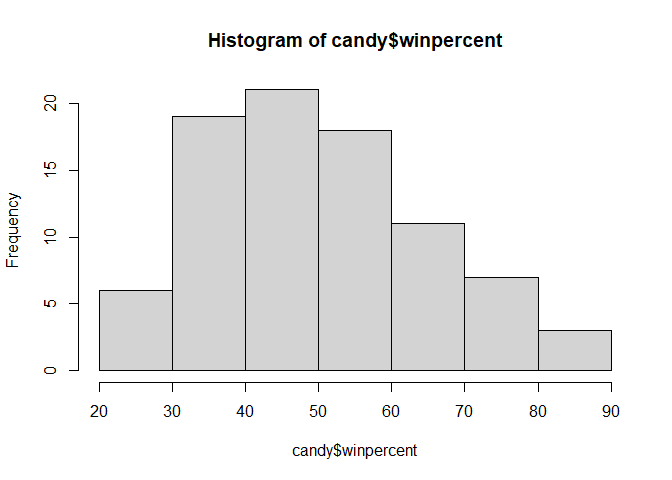
\includegraphics{Class-10_files/figure-latex/unnamed-chunk-9-1.pdf}
\textgreater{} Q9. Is the distribution of winpercent values symmetrical?

The distribution is not symmetrical, it is skewed right

\begin{quote}
Q10. Is the center of the distribution above or below 50\%?
\end{quote}

The center is below 50\%

\begin{quote}
Q11. On average is chocolate candy higher or lower ranked than fruit
candy?
\end{quote}

\begin{Shaded}
\begin{Highlighting}[]
\FunctionTok{mean}\NormalTok{(candy}\SpecialCharTok{$}\NormalTok{winpercent[}\FunctionTok{as.logical}\NormalTok{(candy}\SpecialCharTok{$}\NormalTok{chocolate)]) }\SpecialCharTok{\textgreater{}} \FunctionTok{mean}\NormalTok{(candy}\SpecialCharTok{$}\NormalTok{winpercent[}\FunctionTok{as.logical}\NormalTok{(candy}\SpecialCharTok{$}\NormalTok{fruity)])}
\end{Highlighting}
\end{Shaded}

\begin{verbatim}
## [1] TRUE
\end{verbatim}

Chocolate is ranked higher than fruity candy

\begin{quote}
Q12. Is this difference statistically significant?
\end{quote}

\begin{Shaded}
\begin{Highlighting}[]
\FunctionTok{t.test}\NormalTok{(candy}\SpecialCharTok{$}\NormalTok{winpercent[}\FunctionTok{as.logical}\NormalTok{(candy}\SpecialCharTok{$}\NormalTok{chocolate)], candy}\SpecialCharTok{$}\NormalTok{winpercent[}\FunctionTok{as.logical}\NormalTok{(candy}\SpecialCharTok{$}\NormalTok{fruity)])}
\end{Highlighting}
\end{Shaded}

\begin{verbatim}
## 
##  Welch Two Sample t-test
## 
## data:  candy$winpercent[as.logical(candy$chocolate)] and candy$winpercent[as.logical(candy$fruity)]
## t = 6.2582, df = 68.882, p-value = 2.871e-08
## alternative hypothesis: true difference in means is not equal to 0
## 95 percent confidence interval:
##  11.44563 22.15795
## sample estimates:
## mean of x mean of y 
##  60.92153  44.11974
\end{verbatim}

With this low p value less than 0.05, the difference between chocolate
and fruity candy is significant.

\hypertarget{overall-candy-rankings}{%
\subsection{Overall Candy Rankings}\label{overall-candy-rankings}}

Sort by winpercent \textgreater{} Q13. What are the five least liked
candy types in this set?

\begin{Shaded}
\begin{Highlighting}[]
\FunctionTok{library}\NormalTok{(dplyr)}
\end{Highlighting}
\end{Shaded}

\begin{verbatim}
## 
## Attaching package: 'dplyr'
\end{verbatim}

\begin{verbatim}
## The following objects are masked from 'package:stats':
## 
##     filter, lag
\end{verbatim}

\begin{verbatim}
## The following objects are masked from 'package:base':
## 
##     intersect, setdiff, setequal, union
\end{verbatim}

\begin{Shaded}
\begin{Highlighting}[]
\NormalTok{candy }\SpecialCharTok{\%\textgreater{}\%} 
  \FunctionTok{arrange}\NormalTok{(winpercent) }\SpecialCharTok{\%\textgreater{}\%} 
  \FunctionTok{head}\NormalTok{(}\DecValTok{5}\NormalTok{)}
\end{Highlighting}
\end{Shaded}

\begin{verbatim}
##                    chocolate fruity caramel peanutyalmondy nougat
## Nik L Nip                  0      1       0              0      0
## Boston Baked Beans         0      0       0              1      0
## Chiclets                   0      1       0              0      0
## Super Bubble               0      1       0              0      0
## Jawbusters                 0      1       0              0      0
##                    crispedricewafer hard bar pluribus sugarpercent pricepercent
## Nik L Nip                         0    0   0        1        0.197        0.976
## Boston Baked Beans                0    0   0        1        0.313        0.511
## Chiclets                          0    0   0        1        0.046        0.325
## Super Bubble                      0    0   0        0        0.162        0.116
## Jawbusters                        0    1   0        1        0.093        0.511
##                    winpercent
## Nik L Nip            22.44534
## Boston Baked Beans   23.41782
## Chiclets             24.52499
## Super Bubble         27.30386
## Jawbusters           28.12744
\end{verbatim}

\begin{quote}
Q14. What are the top 5 all time favorite candy types out of this set?
\end{quote}

\begin{Shaded}
\begin{Highlighting}[]
\NormalTok{candy }\SpecialCharTok{\%\textgreater{}\%} 
  \FunctionTok{arrange}\NormalTok{(}\FunctionTok{desc}\NormalTok{(winpercent)) }\SpecialCharTok{\%\textgreater{}\%} 
  \FunctionTok{head}\NormalTok{(}\DecValTok{5}\NormalTok{)}
\end{Highlighting}
\end{Shaded}

\begin{verbatim}
##                            chocolate fruity caramel peanutyalmondy nougat
## ReeseÕs Peanut Butter cup         1      0       0              1      0
## ReeseÕs Miniatures                1      0       0              1      0
## Twix                               1      0       1              0      0
## Kit Kat                            1      0       0              0      0
## Snickers                           1      0       1              1      1
##                            crispedricewafer hard bar pluribus sugarpercent
## ReeseÕs Peanut Butter cup                0    0   0        0        0.720
## ReeseÕs Miniatures                       0    0   0        0        0.034
## Twix                                      1    0   1        0        0.546
## Kit Kat                                   1    0   1        0        0.313
## Snickers                                  0    0   1        0        0.546
##                            pricepercent winpercent
## ReeseÕs Peanut Butter cup        0.651   84.18029
## ReeseÕs Miniatures               0.279   81.86626
## Twix                              0.906   81.64291
## Kit Kat                           0.511   76.76860
## Snickers                          0.651   76.67378
\end{verbatim}

\begin{quote}
Q15. Make a first barplot of candy ranking based on winpercent values.
\end{quote}

\begin{Shaded}
\begin{Highlighting}[]
\FunctionTok{library}\NormalTok{(ggplot2)}
\NormalTok{candy }\SpecialCharTok{\%\textgreater{}\%} 
  \FunctionTok{ggplot}\NormalTok{(}\FunctionTok{aes}\NormalTok{(winpercent, }\FunctionTok{rownames}\NormalTok{(candy))) }\SpecialCharTok{+} 
  \FunctionTok{geom\_col}\NormalTok{()}
\end{Highlighting}
\end{Shaded}

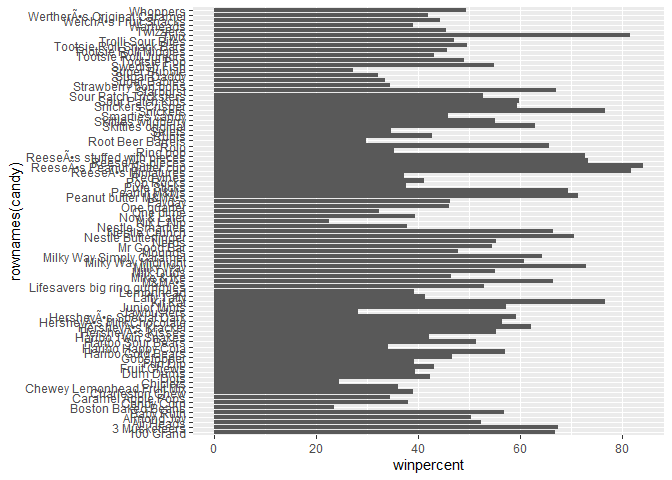
\includegraphics{Class-10_files/figure-latex/unnamed-chunk-14-1.pdf}

\begin{quote}
Q16. This is quite ugly, use the reorder() function to get the bars
sorted by winpercent?
\end{quote}

\begin{Shaded}
\begin{Highlighting}[]
\NormalTok{candy }\SpecialCharTok{\%\textgreater{}\%} 
  \FunctionTok{ggplot}\NormalTok{(}\FunctionTok{aes}\NormalTok{(winpercent, }\FunctionTok{reorder}\NormalTok{(}\FunctionTok{rownames}\NormalTok{(candy),winpercent)))}\SpecialCharTok{+}
  \FunctionTok{geom\_col}\NormalTok{()}
\end{Highlighting}
\end{Shaded}

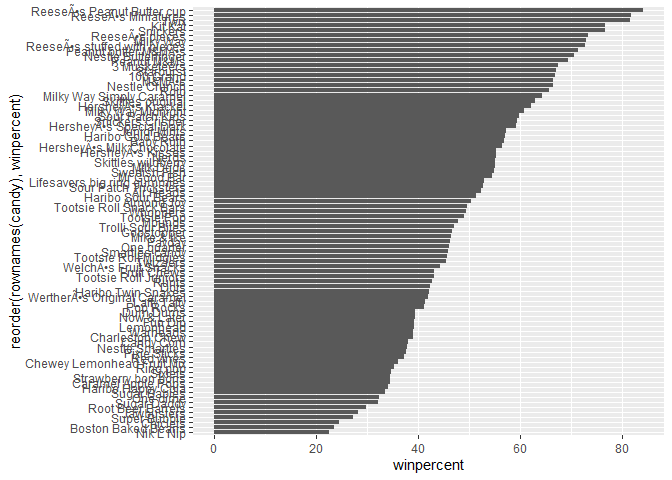
\includegraphics{Class-10_files/figure-latex/unnamed-chunk-15-1.pdf}
Adding color, setting up color vectors

\begin{Shaded}
\begin{Highlighting}[]
\NormalTok{my\_cols}\OtherTok{=}\FunctionTok{rep}\NormalTok{(}\StringTok{"black"}\NormalTok{, }\FunctionTok{nrow}\NormalTok{(candy))}
\NormalTok{my\_cols[}\FunctionTok{as.logical}\NormalTok{(candy}\SpecialCharTok{$}\NormalTok{chocolate)] }\OtherTok{=} \StringTok{"chocolate"}
\NormalTok{my\_cols[}\FunctionTok{as.logical}\NormalTok{(candy}\SpecialCharTok{$}\NormalTok{bar)] }\OtherTok{=} \StringTok{"brown"}
\NormalTok{my\_cols[}\FunctionTok{as.logical}\NormalTok{(candy}\SpecialCharTok{$}\NormalTok{fruity)] }\OtherTok{=} \StringTok{"pink"}
\end{Highlighting}
\end{Shaded}

\begin{Shaded}
\begin{Highlighting}[]
\FunctionTok{ggplot}\NormalTok{(candy) }\SpecialCharTok{+} 
  \FunctionTok{aes}\NormalTok{(winpercent, }\FunctionTok{reorder}\NormalTok{(}\FunctionTok{rownames}\NormalTok{(candy),winpercent)) }\SpecialCharTok{+}
  \FunctionTok{geom\_col}\NormalTok{(}\AttributeTok{fill =}\NormalTok{ my\_cols) }\SpecialCharTok{+}
  \FunctionTok{labs}\NormalTok{(}\AttributeTok{x =} \StringTok{"winpercent"}\NormalTok{, }\AttributeTok{y =} \StringTok{"candy"}\NormalTok{)}
\end{Highlighting}
\end{Shaded}

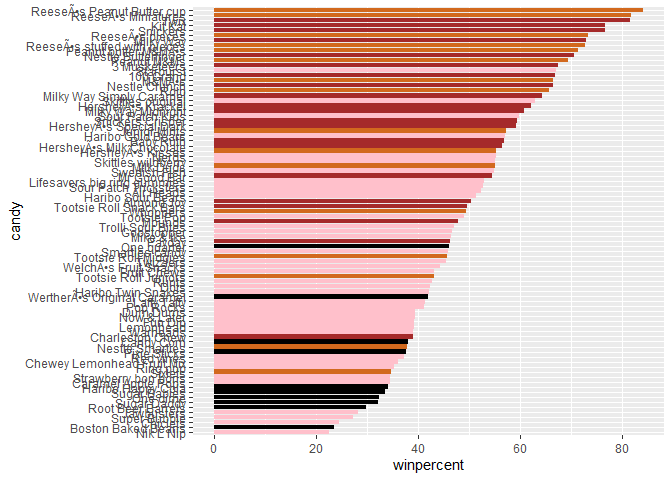
\includegraphics{Class-10_files/figure-latex/unnamed-chunk-17-1.pdf}
\textgreater{} Q17. What is the worst ranked chocolate candy?

Sixlets

\begin{quote}
Q18. What is the best ranked fruity candy?
\end{quote}

Starbursts

\hypertarget{look-at-pricepercent}{%
\subsection{Look at Pricepercent}\label{look-at-pricepercent}}

Fixing the apostrophes

\begin{Shaded}
\begin{Highlighting}[]
\FunctionTok{rownames}\NormalTok{(candy) }\OtherTok{\textless{}{-}} \FunctionTok{gsub}\NormalTok{(}\StringTok{"Õ"}\NormalTok{, }\StringTok{"\textquotesingle{}"}\NormalTok{, }\FunctionTok{rownames}\NormalTok{(candy))}
\end{Highlighting}
\end{Shaded}

\begin{Shaded}
\begin{Highlighting}[]
\FunctionTok{library}\NormalTok{(ggrepel)}
\NormalTok{candy }\SpecialCharTok{\%\textgreater{}\%} 
\FunctionTok{ggplot}\NormalTok{(}\FunctionTok{aes}\NormalTok{(winpercent, pricepercent, }\AttributeTok{label=}\FunctionTok{rownames}\NormalTok{(candy))) }\SpecialCharTok{+}
  \FunctionTok{geom\_point}\NormalTok{(}\AttributeTok{col=}\NormalTok{my\_cols) }\SpecialCharTok{+} 
  \FunctionTok{geom\_text\_repel}\NormalTok{(}\AttributeTok{col=}\NormalTok{my\_cols, }\AttributeTok{size=}\FloatTok{3.3}\NormalTok{, }\AttributeTok{max.overlaps =} \DecValTok{5}\NormalTok{)}
\end{Highlighting}
\end{Shaded}

\begin{verbatim}
## Warning: ggrepel: 54 unlabeled data points (too many overlaps). Consider
## increasing max.overlaps
\end{verbatim}

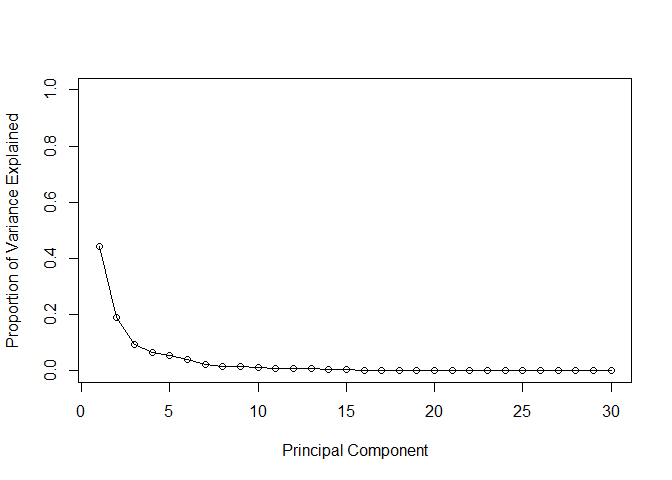
\includegraphics{Class-10_files/figure-latex/unnamed-chunk-19-1.pdf}
\textgreater{} Q19. Which candy type is the highest ranked in terms of
winpercent for the least money - i.e.~offers the most bang for your
buck?

Reese's Miniatures

\begin{quote}
Q20. What are the top 5 most expensive candy types in the dataset and of
these which is the least popular?
\end{quote}

\begin{Shaded}
\begin{Highlighting}[]
\NormalTok{ord }\OtherTok{\textless{}{-}} \FunctionTok{order}\NormalTok{(candy}\SpecialCharTok{$}\NormalTok{pricepercent, }\AttributeTok{decreasing =} \ConstantTok{TRUE}\NormalTok{)}
\FunctionTok{head}\NormalTok{( candy[ord,}\FunctionTok{c}\NormalTok{(}\DecValTok{11}\NormalTok{,}\DecValTok{12}\NormalTok{)], }\AttributeTok{n=}\DecValTok{5}\NormalTok{ )}
\end{Highlighting}
\end{Shaded}

\begin{verbatim}
##                          pricepercent winpercent
## Nik L Nip                       0.976   22.44534
## Nestle Smarties                 0.976   37.88719
## Ring pop                        0.965   35.29076
## Hershey's Krackel               0.918   62.28448
## Hershey's Milk Chocolate        0.918   56.49050
\end{verbatim}

Out of these top five most expensive, Nik L Nip is the least popular

\hypertarget{lollipop-chart-of-pricepercent}{%
\subsection{Lollipop chart of
pricepercent}\label{lollipop-chart-of-pricepercent}}

\begin{Shaded}
\begin{Highlighting}[]
\NormalTok{candy }\SpecialCharTok{\%\textgreater{}\%} 
  \FunctionTok{ggplot}\NormalTok{(}\FunctionTok{aes}\NormalTok{(pricepercent, }\FunctionTok{reorder}\NormalTok{(}\FunctionTok{rownames}\NormalTok{(candy), pricepercent))) }\SpecialCharTok{+}
  \FunctionTok{geom\_segment}\NormalTok{(}\FunctionTok{aes}\NormalTok{(}\AttributeTok{yend =} \FunctionTok{reorder}\NormalTok{(}\FunctionTok{rownames}\NormalTok{(candy), pricepercent), }
                   \AttributeTok{xend =} \DecValTok{0}\NormalTok{), }\AttributeTok{col=}\StringTok{"gray40"}\NormalTok{) }\SpecialCharTok{+}
    \FunctionTok{geom\_point}\NormalTok{()}\SpecialCharTok{+}
  \FunctionTok{labs}\NormalTok{(}\AttributeTok{x =} \StringTok{"Price"}\NormalTok{, }\AttributeTok{y =} \StringTok{"Candy"}\NormalTok{)}
\end{Highlighting}
\end{Shaded}

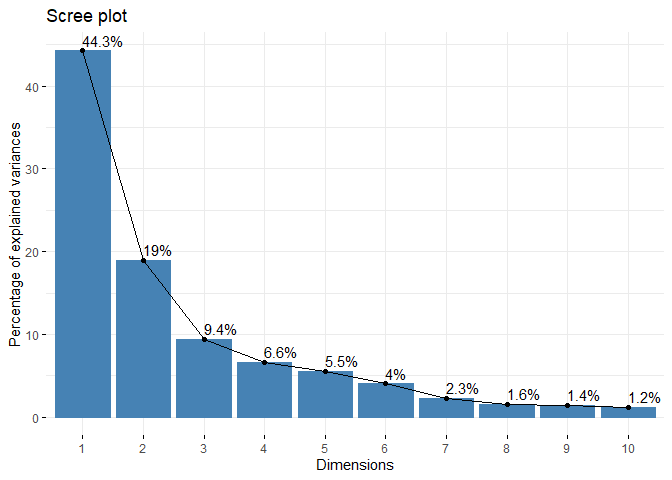
\includegraphics{Class-10_files/figure-latex/unnamed-chunk-21-1.pdf}

\hypertarget{exploring-the-correlation-structure}{%
\subsection{Exploring the Correlation
Structure}\label{exploring-the-correlation-structure}}

Exploring how the variables interact with each other using correlation

\begin{Shaded}
\begin{Highlighting}[]
\FunctionTok{library}\NormalTok{(corrplot)}
\end{Highlighting}
\end{Shaded}

\begin{verbatim}
## corrplot 0.90 loaded
\end{verbatim}

\begin{Shaded}
\begin{Highlighting}[]
\NormalTok{cij }\OtherTok{\textless{}{-}} \FunctionTok{cor}\NormalTok{(candy)}
\FunctionTok{corrplot}\NormalTok{(cij)}
\end{Highlighting}
\end{Shaded}

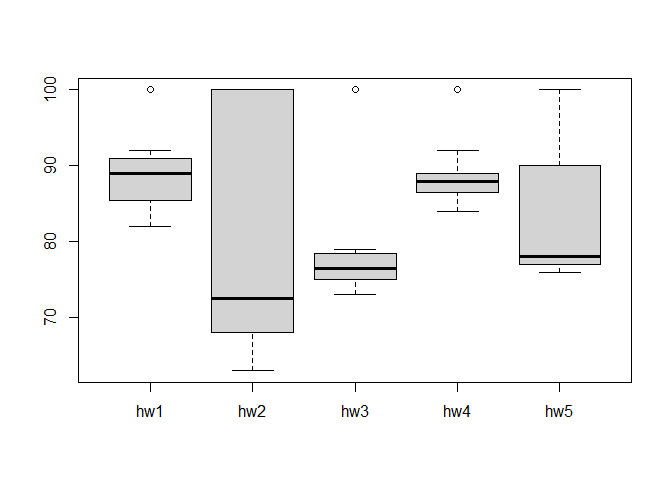
\includegraphics{Class-10_files/figure-latex/unnamed-chunk-23-1.pdf}
\textgreater{} Q22. Examining this plot what two variables are
anti-correlated (i.e.~have minus values)?

Fruity/chocolate and bar/pluribus are anti-correlated

\begin{quote}
Q23. Similarly, what two variables are most positively correlated?
\end{quote}

Chocolate/winpercent and chocolate/bar are the most positively
correlated

\hypertarget{principal-component-analysis}{%
\subsection{Principal Component
Analysis}\label{principal-component-analysis}}

Time to apply PCA!

\begin{Shaded}
\begin{Highlighting}[]
\NormalTok{pca }\OtherTok{\textless{}{-}} \FunctionTok{prcomp}\NormalTok{(candy, }\AttributeTok{scale =} \ConstantTok{TRUE}\NormalTok{)}
\FunctionTok{summary}\NormalTok{(pca)}
\end{Highlighting}
\end{Shaded}

\begin{verbatim}
## Importance of components:
##                           PC1    PC2    PC3     PC4    PC5     PC6     PC7
## Standard deviation     2.0788 1.1378 1.1092 1.07533 0.9518 0.81923 0.81530
## Proportion of Variance 0.3601 0.1079 0.1025 0.09636 0.0755 0.05593 0.05539
## Cumulative Proportion  0.3601 0.4680 0.5705 0.66688 0.7424 0.79830 0.85369
##                            PC8     PC9    PC10    PC11    PC12
## Standard deviation     0.74530 0.67824 0.62349 0.43974 0.39760
## Proportion of Variance 0.04629 0.03833 0.03239 0.01611 0.01317
## Cumulative Proportion  0.89998 0.93832 0.97071 0.98683 1.00000
\end{verbatim}

Time to plot

\begin{Shaded}
\begin{Highlighting}[]
\FunctionTok{plot}\NormalTok{(pca}\SpecialCharTok{$}\NormalTok{x[,}\DecValTok{1}\SpecialCharTok{:}\DecValTok{2}\NormalTok{])}
\end{Highlighting}
\end{Shaded}

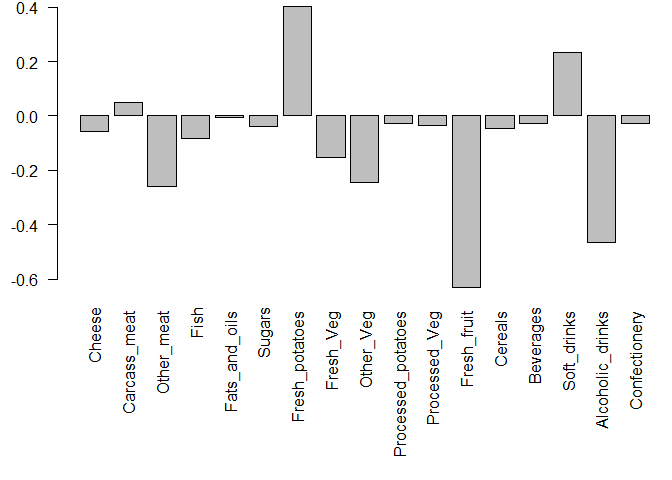
\includegraphics{Class-10_files/figure-latex/unnamed-chunk-25-1.pdf}

\begin{Shaded}
\begin{Highlighting}[]
\FunctionTok{plot}\NormalTok{(pca}\SpecialCharTok{$}\NormalTok{x[,}\DecValTok{1}\SpecialCharTok{:}\DecValTok{2}\NormalTok{], }\AttributeTok{col =}\NormalTok{ my\_cols, }\AttributeTok{pch =} \DecValTok{16}\NormalTok{)}
\end{Highlighting}
\end{Shaded}

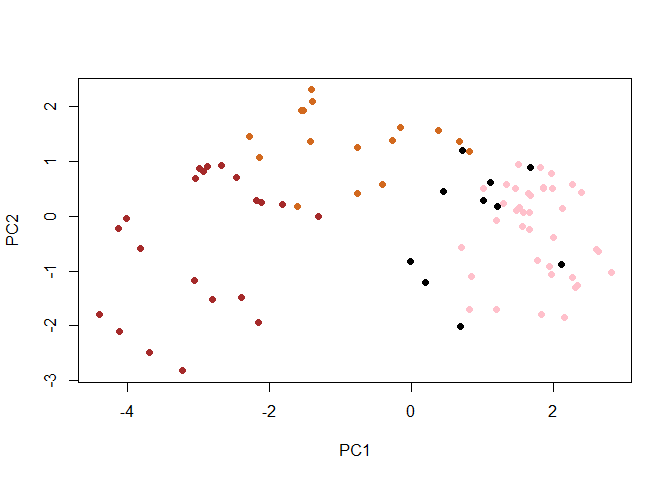
\includegraphics{Class-10_files/figure-latex/unnamed-chunk-26-1.pdf} Try
using ggplot2 First, make a dataframe

\begin{Shaded}
\begin{Highlighting}[]
\NormalTok{my\_data }\OtherTok{\textless{}{-}} \FunctionTok{cbind}\NormalTok{(candy, pca}\SpecialCharTok{$}\NormalTok{x[,}\DecValTok{1}\SpecialCharTok{:}\DecValTok{3}\NormalTok{])}
\end{Highlighting}
\end{Shaded}

\begin{Shaded}
\begin{Highlighting}[]
\NormalTok{p }\OtherTok{\textless{}{-}}\NormalTok{ my\_data }\SpecialCharTok{\%\textgreater{}\%} 
  \FunctionTok{ggplot}\NormalTok{(}\FunctionTok{aes}\NormalTok{(}\AttributeTok{x =}\NormalTok{ PC1, }\AttributeTok{y =}\NormalTok{ PC2, }\AttributeTok{size =}\NormalTok{ winpercent}\SpecialCharTok{/}\DecValTok{100}\NormalTok{, }\AttributeTok{text =} \FunctionTok{rownames}\NormalTok{(my\_data), }\AttributeTok{label =} \FunctionTok{rownames}\NormalTok{(my\_data))) }\SpecialCharTok{+}
  \FunctionTok{geom\_point}\NormalTok{(}\AttributeTok{col =}\NormalTok{ my\_cols)}
\NormalTok{p}
\end{Highlighting}
\end{Shaded}

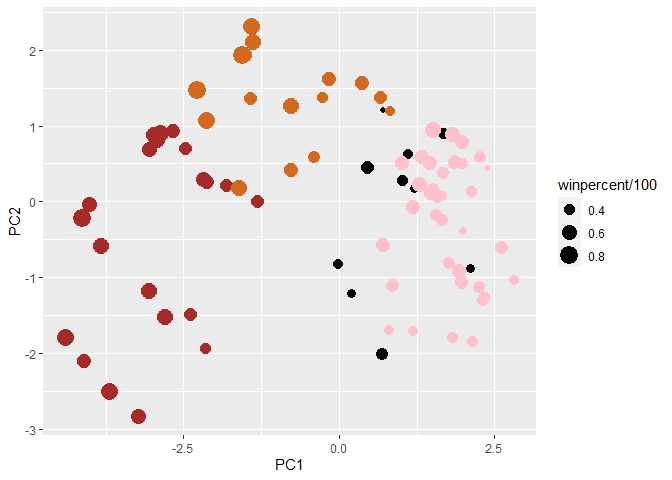
\includegraphics{Class-10_files/figure-latex/unnamed-chunk-28-1.pdf}

Use the ggrepel package to label the graph

\begin{Shaded}
\begin{Highlighting}[]
\FunctionTok{library}\NormalTok{(ggrepel)}
\NormalTok{p }\SpecialCharTok{+} \FunctionTok{geom\_text\_repel}\NormalTok{(}\AttributeTok{size=}\FloatTok{3.3}\NormalTok{, }\AttributeTok{col=}\NormalTok{my\_cols, }\AttributeTok{max.overlaps =} \DecValTok{7}\NormalTok{)  }\SpecialCharTok{+} 
  \FunctionTok{theme}\NormalTok{(}\AttributeTok{legend.position =} \StringTok{"none"}\NormalTok{) }\SpecialCharTok{+}
  \FunctionTok{labs}\NormalTok{(}\AttributeTok{title=}\StringTok{"Halloween Candy PCA Space"}\NormalTok{,}
       \AttributeTok{subtitle=}\StringTok{"Colored by type: chocolate bar (dark brown), chocolate other (light brown), fruity (red), other (black)"}\NormalTok{,}
       \AttributeTok{caption=}\StringTok{"Data from 538"}\NormalTok{)}
\end{Highlighting}
\end{Shaded}

\begin{verbatim}
## Warning: ggrepel: 44 unlabeled data points (too many overlaps). Consider
## increasing max.overlaps
\end{verbatim}

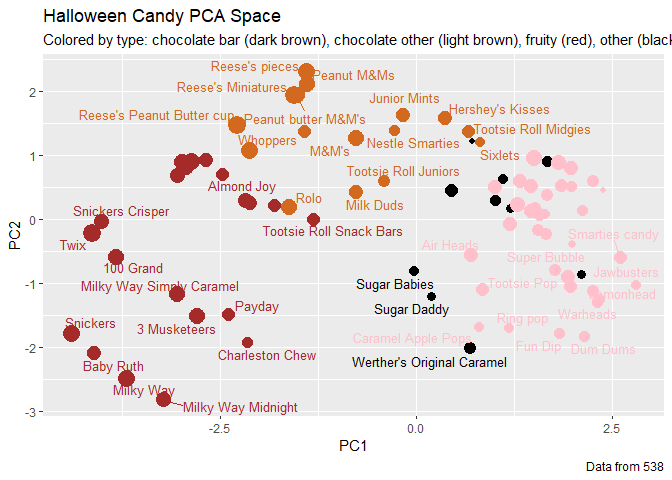
\includegraphics{Class-10_files/figure-latex/unnamed-chunk-29-1.pdf} To
be able to see more labels, use plotly to make interactive \textbf{Must
comment out before printing pdf}

\begin{Shaded}
\begin{Highlighting}[]
\CommentTok{\#library(plotly)}
\end{Highlighting}
\end{Shaded}

\begin{Shaded}
\begin{Highlighting}[]
\CommentTok{\#ggplotly(p)}
\end{Highlighting}
\end{Shaded}

Looking ar our PCA loadings. Should have opposite bars on variables we
know do not correlate with each other

\begin{Shaded}
\begin{Highlighting}[]
\FunctionTok{par}\NormalTok{(}\AttributeTok{mar=}\FunctionTok{c}\NormalTok{(}\DecValTok{8}\NormalTok{,}\DecValTok{4}\NormalTok{,}\DecValTok{2}\NormalTok{,}\DecValTok{2}\NormalTok{))}
\FunctionTok{barplot}\NormalTok{(pca}\SpecialCharTok{$}\NormalTok{rotation[,}\DecValTok{1}\NormalTok{], }\AttributeTok{las=}\DecValTok{2}\NormalTok{, }\AttributeTok{ylab=}\StringTok{"PC1 Contribution"}\NormalTok{)}
\end{Highlighting}
\end{Shaded}

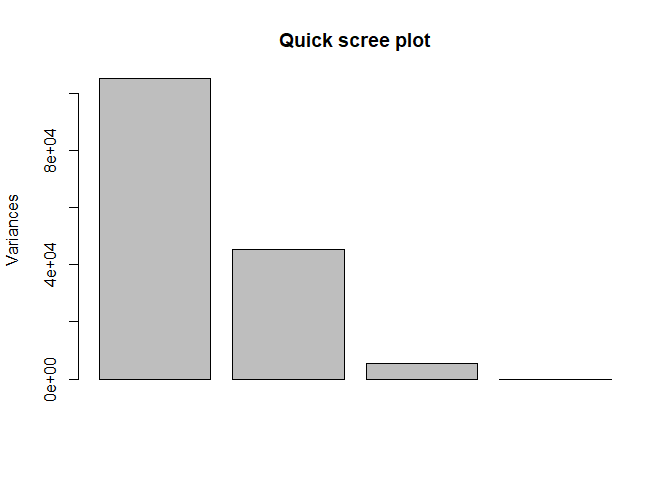
\includegraphics{Class-10_files/figure-latex/unnamed-chunk-32-1.pdf}

\begin{quote}
Q24. What original variables are picked up strongly by PC1 in the
positive direction? Do these make sense to you?
\end{quote}

Fruity, hard, and bar, are picked up strongly by the PC1 component which
makes sense because, when looking at the correlation matrix, these
variables did not positively correlate with many of the other variables.
Also, these three variables correlated positively with each other, so it
makes sense that they are all on the same side of the loadings plot.

\end{document}
